\documentclass[hidelinks,12pt]{article}
\usepackage[left=0.25cm,top=1cm,right=0.25cm,bottom=1cm]{geometry}
%\usepackage[landscape]{geometry}
\textwidth = 20cm
\hoffset = -1cm
\usepackage[utf8]{inputenc}
\usepackage[spanish,es-tabla]{babel}
\usepackage[autostyle,spanish=mexican]{csquotes}
\usepackage[tbtags]{amsmath}
\usepackage{nccmath}
\usepackage{amsthm}
\usepackage{amssymb}
\usepackage{mathrsfs}
\usepackage{graphicx}
\usepackage{subfig}
\usepackage{standalone}
\usepackage[outdir=./Imagenes/]{epstopdf}
\usepackage{siunitx}
\usepackage{physics}
\usepackage{color}
\usepackage{float}
\usepackage{hyperref}
\usepackage{multicol}
%\usepackage{milista}
\usepackage{anyfontsize}
\usepackage{anysize}
%\usepackage{enumerate}
\usepackage[shortlabels]{enumitem}
\usepackage{capt-of}
\usepackage{bm}
\usepackage{relsize}
\usepackage{placeins}
\usepackage{empheq}
\usepackage{cancel}
\usepackage{wrapfig}
\usepackage[flushleft]{threeparttable}
\usepackage{makecell}
\usepackage{fancyhdr}
\usepackage{tikz}
\usepackage{bigints}
\usepackage{scalerel}
\usepackage{pgfplots}
\usepackage{pdflscape}
\pgfplotsset{compat=1.16}
\spanishdecimal{.}
\renewcommand{\baselinestretch}{1.5} 
\renewcommand\labelenumii{\theenumi.{\arabic{enumii}})}
\newcommand{\ptilde}[1]{\ensuremath{{#1}^{\prime}}}
\newcommand{\stilde}[1]{\ensuremath{{#1}^{\prime \prime}}}
\newcommand{\ttilde}[1]{\ensuremath{{#1}^{\prime \prime \prime}}}
\newcommand{\ntilde}[2]{\ensuremath{{#1}^{(#2)}}}

\newtheorem{defi}{{\it Definición}}[section]
\newtheorem{teo}{{\it Teorema}}[section]
\newtheorem{ejemplo}{{\it Ejemplo}}[section]
\newtheorem{propiedad}{{\it Propiedad}}[section]
\newtheorem{lema}{{\it Lema}}[section]
\newtheorem{cor}{Corolario}
\newtheorem{ejer}{Ejercicio}[section]

\newlist{milista}{enumerate}{2}
\setlist[milista,1]{label=\arabic*)}
\setlist[milista,2]{label=\arabic{milistai}.\arabic*)}
\newlength{\depthofsumsign}
\setlength{\depthofsumsign}{\depthof{$\sum$}}
\newcommand{\nsum}[1][1.4]{% only for \displaystyle
    \mathop{%
        \raisebox
            {-#1\depthofsumsign+1\depthofsumsign}
            {\scalebox
                {#1}
                {$\displaystyle\sum$}%
            }
    }
}
\def\scaleint#1{\vcenter{\hbox{\scaleto[3ex]{\displaystyle\int}{#1}}}}
\def\bs{\mkern-12mu}


\usepackage{apacite}

\AtBeginDocument{\RenewCommandCopy\qty\SI}
\ExplSyntaxOn
\msg_redirect_name:nnn { siunitx } { physics-pkg } { none }
\ExplSyntaxOff

\title{2 - Diferenciales y operadores diferenciales \\[0.3em]  \large{Matemáticas Avanzadas de la Física}\vspace{-3ex}}
\author{M. en C. Gustavo Contreras Mayén}
\date{ }

\begin{document}
\vspace{-4cm}
\maketitle
\fontsize{14}{14}\selectfont
\tableofcontents
\newpage

\section{Diferencial de línea.}

\subsection{Construcción.}

Utilizando el resultado que define a un vector unitario en un sistema coordenado curvilíneo:
\begin{align*}
\vu{e}_{i} = \dfrac{1}{h_{i}} \, \pdv{\vb{r}}{u_{i}}
\end{align*}
para las componentes vectoriales:
\begin{align*}
\dd{\vb{r}} = \nsum_{i=1}^{3} \pdv{\vb{r}}{u_{i}} \dd{u_{i}}
\end{align*}
Es posible escribir:
\begin{align}
\dd{\vb{r}} = \nsum_{i=1}^{3} h_{i} \, \vu{e}_{i} \dd{u_{i}} = \nsum_{i=1}^{3} \dd{\vb{l}_{i}}
\label{eq:ecuacion_01_21}
\end{align}
donde:
\begin{align}
\dd{\vb{l}_{i}} = h_{i} \, \vu{e}_{i} \dd{u_{i}}
\label{eq:ecuacion_01_22}
\end{align}
que representa el \emph{elemento diferencial de línea} a lo largo del eje $u_{i}$.
\par
La ec. (\ref{eq:ecuacion_01_22}) asegura que cualquier elemento de línea con orientación arbitraria, puede descomponerse en una suma vectorial.

\subsection{Coordenadas esféricas.}

En coordenadas esféricas (ocupando los factores de escala ya conocidos) tenemos que:
\begin{table}[H]
\centering
\fontsize{14}{14}\selectfont
\begin{tabular}{r  c  l}
$\dd{\vb{l}_{r}} = \vu{e}_{r} \dd{r}$ & $\longrightarrow$ & $\dd{l_{r}} = \dd{r}$ \\
$\dd{\vb{l}_{\theta}} = \vu{e}_{\theta} \, r \dd{\theta}$ & $\longrightarrow$ & $\dd{l_{\theta}} = r \, \dd{\theta}$ \\
$\dd{\vb{l}_{\varphi}} = \vu{e}_{\varphi} \, r \, \sin \theta \dd{\varphi}$ & $\longrightarrow$ & $\dd{l_{\varphi}} = r \, \sin \theta \dd{\varphi}$ \\
\end{tabular}
\end{table}

\section{Diferencial de superficie.}

\subsection{Construcción.}

Las superficies diferenciales se describen como vectores perpendicular al área diferencial, como se ve en la siguiente figura (\ref{fig:figura_diferenciales_superficie}):

\begin{figure}[h!]
    \centering
    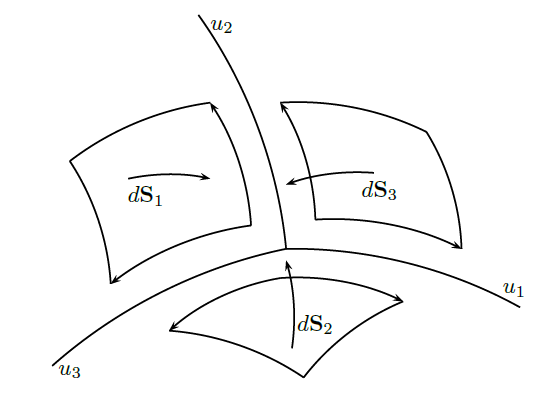
\includegraphics[scale=0.75]{Imagenes/Diferenciales_Superficie_01.png}
    \caption{Elementos diferenciales de área en coordenadas curvilíneas, los vectores mostrados son perpendiculares a su superficie.}
    \label{fig:figura_diferenciales_superficie}
\end{figure}

Las superficies están orientadas según la regla de la mano derecha, por lo que:
\begin{align*}
\dd{\vb{S}_{1}} &= \dd{\vb{l}_{2}} \cp \dd{\vb{l}_{3}} \\[0.5em] 
\dd{\vb{S}_{2}} &= \dd{\vb{l}_{3}} \cp \dd{\vb{l}_{1}} \\[0.5em]
\dd{\vb{S}_{3}} &= \dd{\vb{l}_{1}} \cp \dd{\vb{l}_{2}}
\end{align*}

Usando las relaciones:
\begin{align*}
\vu{e}_{1} \cp \vu{e}_{2} = \vu{e}_{3} \\
\vu{e}_{2} \cp \vu{e}_{3} = \vu{e}_{1} \\
\vu{e}_{3} \cp \vu{e}_{1} = \vu{e}_{2}
\end{align*}
que son válidas para sistemas coordenados curvilíneos ortonormales, en espacios $\mathbb{R}^{3}$ euclidianos.
\par
Que en forma sintética queda expresado por:
\begin{align}
\vu{e}_{i} \cp \vu{e}_{j} = \nsum_{i=1}^{3} \epsilon_{ijk} \, \vu{e}_{k}
\end{align}
donde $\epsilon_{ijk}$ es el símbolo de \emph{Levi-Civita} que definimos en la presentación anterior. Así encontramos que:
\begin{align*}
\dd{\vb{S}_{1}} &= h_{2} \, h_{3} \, \vu{e}_{2} \cp \vu{e}_{3} \dd{u_{2}} \dd{u_{3}} = \\[0.5em]
&= h_{2} \, h_{3} \, \vu{e}_{1} \dd{u_{2}} \dd{u_{3}} = \\[0.5em]
&= \vu{e}_{1} \dd{S_{1}}
\end{align*}

Para los otros dos diferenciales de superficie:
\begin{align*}
\dd{\vb{S}_{2}} &= h_{3} \, h_{1} \, \vu{e}_{3} \cp \vu{e}_{1} \dd{u_{3}} \dd{u_{1}} = \\[0.5em]
&= h_{3} \, h_{1} \, \vu{e}_{2} \dd{u_{3}} \dd{u_{1}} = \\[0.5em]
&= \vu{e}_{2} \dd{S_{2}} \\[1em]
\dd{\vb{S}_{3}} &= h_{1} \, h_{2} \, \vu{e}_{1} \cp \vu{e}_{2} \dd{u_{1}} \dd{u_{2}} = \\[0.5em]
&= h_{1} \, h_{2} \, \vu{e}_{3} \dd{u_{1}} \dd{u_{2}} = \\[0.5em]
&= \vu{e}_{3} \dd{S_{3}}
\end{align*}

\section{Diferencial de volumen.}

\subsection{Construcción.}

El elemento diferencial de volumen se define como:
\begin{align*}
\dd{V} &= \dd{\vb{l}_{1}} \cdot \dd{\vb{l}_{2}} \cp \dd{\vb{l}_{3}} = \\
&= h_{1} \, h_{2} \, h_{3} \, \vu{e}_{1} \cdot \vu{e}_{2} \cp \vu{e}_{3} \dd{u_{1}} \dd{u_{2}} \dd{u_{3}} = \\
&= h_{1} \, h_{2} \, h_{3} \dd{u_{1}} \dd{u_{2}} \dd{u_{3}}
\end{align*}

\subsection{Coordenadas esféricas.}

En coordenadas esféricas tenemos:
\begin{align*}
\dd{S_{1}} &= \dd{S_{r}} = h_{\theta} \, h_{\varphi} \dd{\theta} \dd{\varphi} = r^{2} \sin \theta \dd{\theta} \dd{\varphi} \\[0.5em]
\dd{S_{2}} &= \dd{S_{\theta}} = h_{\varphi} \, h_{r} \dd{\varphi} \dd{r} = r \sin \theta \dd{\theta} \dd{\varphi} \\[0.5em]
\dd{S_{3}} &= \dd{S_{\varphi}} = h_{r} \, h_{\theta} \dd{r} \dd{\theta} = r \dd{r} \dd{\theta}
\end{align*}

Entonces el diferencial de volumen es:
\begin{align*}
\dd{V} &= h_{r} \, h_{\theta} \, h_{\varphi} \dd{r} \dd{\theta} \dd{\varphi} = \\[0.5em]
&= r^{2} \, \sin \theta \dd{r} \dd{\theta} \dd{\varphi}
\end{align*}

% \textbf{Ejercicio a cuenta (2). } La velocidad y la aceleración se definen en la forma vectorial como:
% \begin{align*}
% \vb{v} = \dv{\vb{r}}{t} = \dot{\vb{r}} \hspace{1cm} \vb{a} = \dot{\vb{v}} = \ddot{\vb{r}}
% \end{align*}
% Calcula para el sistema coordenado esférico:
% \begin{enumerate}
% \item $\dot{\vu{e}}_{r}$, $\dot{\vu{e}}_{\theta}$, $\dot{\vu{e}}_{\varphi}$ 
% \item La velocidad $\vb{v}$.
% \item La aceleración $\vb{a}$.
% \end{enumerate}

% \textbf{Ejercicio a cuenta (3). } Utilizando notación de índices, demuestra que con los vectores\footnote{Recuerda que como se ha comentado, la representación de un vector es: $\vb{A} = \va{A}$.} $\vb{A}$,  $\vb{B}$, $\vb{C}$ y $\vb{D}$, se cumplen las identidades:
% \begin{enumerate}
% \item $(\vb{A} \cp \vb{B}) \cdot (\vb{C} \cp \vb{D}) = (\vb{A} \cdot \vb{C})(\vb{B} \cdot \vb{D}) - (\vb{A} \cdot \vb{D})(\vb{B} \cdot \vb{C})$
% \item $\vb{A} \cp (\vb{B} \cp \vb{C}) + \vb{B} \cp (\vb{C} \cp \vb{A}) + \vb{C} \cp (\vb{A} \cp \vb{B}) = \va{0}$
% \end{enumerate}

\newpage
\section{Operadores diferenciales.}

\subsection{Características de los campos.}

En la presentación anterior mencionamos la naturaleza de los campos escalares y vectoriales.
\par
Asumiremos que los campos son funciones regulares, continuas y derivables, excepto posiblemente en algunos puntos aislados. En general los campos serán descritos por ecuaciones diferenciales parciales cuyas variables independientes serán la posición y el tiempo.

\subsection{Gradiente.}

\subsubsection{Definición.}

Al pasar de un punto:
\begin{align*}
P(u_{1}, u_{2}, u_{3})
\end{align*}
a otro infinitesimalmente cercano:
\begin{align*}
P(u_{1} + \dd{u}_{1}, u_{2} + \dd{u_{2}} + u_{3} + \dd{u_{3}})
\end{align*}
El cambio diferencial de una función (o campo) escalar $\phi(u_{1}, u_{2}, u_{3})$ está dado por:
\begin{align}
\begin{aligned}
\dd{\phi} &= \pdv{\phi}{u_{1}} \dd{u_{1}} + \pdv{\phi}{u_{2}} \dd{u_{2}} + \pdv{\phi}{u_{3}} \dd{u_{3}} \\[0.5em]
&= \nsum_{i=1}^{3} \pdv{\phi}{u_{i}} \dd{u_{i}}
\end{aligned}
\label{eq:ecuacion_01_26}
\end{align}
Teniendo en cuenta la ec. (\ref{eq:ecuacion_01_21}) se sigue que:
\begin{align}
\dd{\vb{r}} = \nsum_{j=1}^{3} h_{j} \, \vu{e}_{j} \dd{u_{j}}
\label{eq:ecuacion_01_27}
\end{align}
Multiplicando escalarmente por $\vu{e}_{i}$ tenemos que:
\begin{align*}
\dd{\vb{r}} \cdot \vu{e}_{i} &= \nsum_{j=1}^{3} h_{j} \, \vu{e}_{j} \cdot \vu{e}_{j} \dd{u_{j}} = \nsum_{j=1}^{3} h_{j} \, \delta_{ij} \dd{u_{j}} \\[0.5em]
&= h_{i} \dd{u_{i}} \\[1em]
&\Longrightarrow \dd{u_{i}} = \dfrac{1}{h_{i}} \dd{\vb{r}} \cdot \vu{e}_{i}
\end{align*}
Al sustituir en la ec. (\ref{eq:ecuacion_01_26}), llegamos a:
\begin{align*}
\dd{\phi} &= \nsum_{i=1}^{3} \pdv{\phi}{u_{i}} \, \dfrac{1}{h_{i}} \, \vu{e}_{i} \cdot \dd{\vb{r}} = \\[0.5em]
&= \dd{\vb{r}} \cdot \left( \nsum_{i=1}^{3} \dfrac{\vu{e_{i}}}{h_{i}} \, \pdv{\phi}{u_{i}} \right)
\end{align*}
Al término entre paréntesis lo denotamos $\grad{\phi}$.
\par
El operador \emph{nabla} es:
\begin{align}
\grad{\phi} = \nsum_{i=1}^{3} \dfrac{\vu{e_{i}}}{h_{i}} \, \pdv{\phi}{u_{i}} = \nsum_{i=1}^{3} \vu{e}_{i} \left( \grad{\phi} \right)_{i}
\label{eq:ecuacion_01_28}
\end{align}
Se le llamará \emph{gradiente de la función escalar} $\phi(u_{i})$, por tanto:
\begin{align}
\dd{\phi} = \dd{\vb{r}} \cdot \grad{\phi}
\label{eq:ecuacion_01_29}
\end{align}
Como tenemos que:
\begin{align*}
\dd{\vb{r}} = \vu{n} \dd{l}
\end{align*}
Se sigue entonces:
\begin{align*}
\dv{\phi}{l} = \vu{n} \cdot \grad{\phi}
\end{align*}
que corresponde a la definición de \emph{derivada direccional} de la función $\phi$ en la dirección de $\vu{n}$.

\subsubsection{Propiedades del gradiente.}

Para estudiar las propiedades del gradiente tomemos un par de superficies infinitesimalmente cercanas, sobre cada una de las cuales la función $\phi$ toma valores constantes e infinitesimalmente distintos: $\phi$ y $\phi + \dd{\phi}$. En la teoría de campos se les llama \emph{superficies equipotenciales}.

\begin{figure}[H]
    \centering
    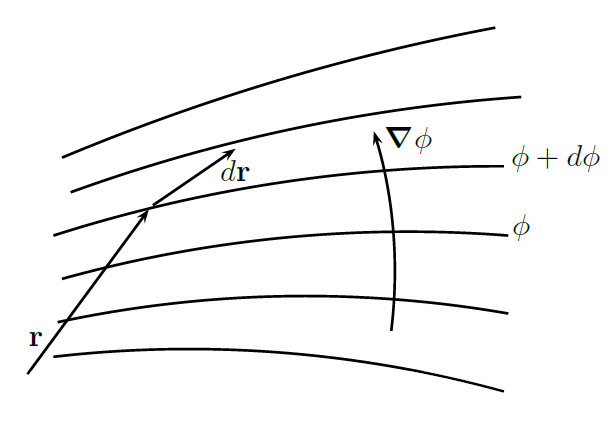
\includegraphics[scale=0.75]{Imagenes/Superficies_Equipotenciales.png}
    \caption{Superficies equipotenciales.}
    \label{fig:Superficies_Equipotenciales}
\end{figure}

De la ec. (\ref{eq:ecuacion_01_29}) se tiene que:
\begin{align*}
\dd{\phi} = \dd{\vb{u}} \cdot \grad{\phi} = \abs{\dd{\vb{r}}} \, \abs{\grad{\phi}} \, \cos \theta
\end{align*}
donde $\theta$ es el ángulo entre $\dd{\vb{r}}$ y $\grad{\phi}$.

Si el vector $\dd{\vb{r}}$ se sitúa en el plano $\phi = \mbox{ constante}$, entonces: $\dd{\phi} = 0$, por lo que
\begin{align*}
0 = \abs{\dd{\vb{r}}} \, \abs{\grad{\phi}} \, \cos \theta
\end{align*}

Como $\grad{\phi}$ es en general diferente de cero, ya que $\phi(u_{i})$ es una función arbitraria, y como $\abs{\dd{\vb{r}}} \neq 0$, se sigue que $\cos \theta = 0$, entonces $\theta = \ang{90}$

En consecuencia: $\grad{\phi}$ es \emph{perpendicular} a la superficie $\phi = \mbox{ constante}$.
\par
El valor máximo de $\dd{\phi}$ se presenta cuando $\theta = 0$, es decir:
\begin{align*}
\dd{\theta}_{\max} &= \abs{\grad{\phi}} \, \abs{\dd{\vb{r}}} \dd{l} \\[1em]
\mbox{o cuando } \hspace{0.5cm} \left( \dv{\phi}{l} \right)_{\max} &= \abs{\grad{\phi}}
\end{align*}

Entonces el módulo del gradiente corresponde al valor máximo de la derivada direccional y el gradiente apunta en la dirección en que tal derivada es máxima.
\par
Dado que para cada punto de una línea o superficie equipotencial es posible trazar el vector $\grad{\phi}$, entonces es posible construir una red coordenada ortogonal a las equipotenciales.
\par
Por lo que, dada una familia de curvas en el plano (o de superficies curvas en el espacio), es posible obtener otras que le sean ortogonales.
\par
Por lo que tenemos un método eficaz de construcción de sistemas de coordenadas curvilíneas ortogonales.
\par
Hay que tomar en cuenta que $\grad$ \emph{no} es un vector, sino un \emph{operador vectorial}: $\grad$ no tiene dirección, a menos que opere sobre una función.
% \\[1em]
% Para ejercitar el avance que llevamos, resuelve los siguientes ejercicios a cuenta:
% \\
% \noindent
% \textbf{Ejercicio a cuenta (4). } Demuestra que $\grad{\phi \psi} = \phi \, \grad{\psi} + \psi \, \grad{\phi}$
% \\
% \noindent
% \textbf{Ejercicio a cuenta (5). } Si $f = f(r)$ con $r = \sqrt{x^{2} + y^{2}+ z^{2}}$, demuestra que:
% \begin{align*}
% \grad{f(r)} = \vu{r} \, \dv{f(r)}{r}
% \end{align*}

\subsection{Divergencia.}

\subsubsection{Flujo de campo vectorial.}

Dada una superficie diferencial orientada $\dd{\vb{S}}$ (figura \ref{fig:figura_superficie_diferencial}), se define el \emph{flujo} del campo vectorial $\vb{B}$ a través de $\dd{\vb{S}}$ como:
\begin{align*}
\mbox{flujo diferencial } = \dd{\Phi} = \vb{B} \cdot \dd{\vb{S}}
\end{align*}

\begin{minipage}{0.5\linewidth}
\begin{figure}[H]
    \centering
    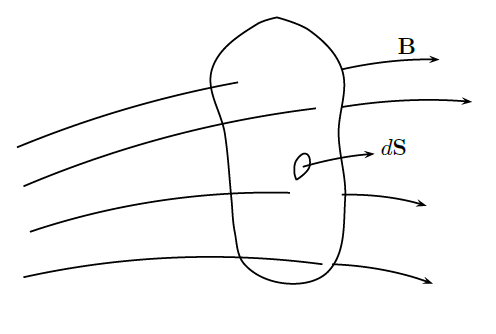
\includegraphics[scale=0.5]{Imagenes/Superficie_Diferencial.png}
    \caption{Flujo del campo $\vb{B}$ a través de una superficie abierta.}
    \label{fig:figura_superficie_diferencial}
\end{figure}
\end{minipage}
\hspace{0.75cm}
\begin{minipage}{0.4\linewidth}
El flujo es máximo si \\ $\vb{B} \parallel \dd{\vb{S}}$ y es nulo si $\vb{B} \bot \dd{\vb{S}}$.
\end{minipage}
\\[1.5em]
Nos enfocaremos en el cálculo del flujo a través de una superficie diferencial \emph{cerrada}, que contenga un volumen diferencial $\dd{V}$ limitado por superficies coordenadas.
\par
El volumen será entonces un paralelepípedo curvilíneo:
\begin{figure}[H]
    \centering
    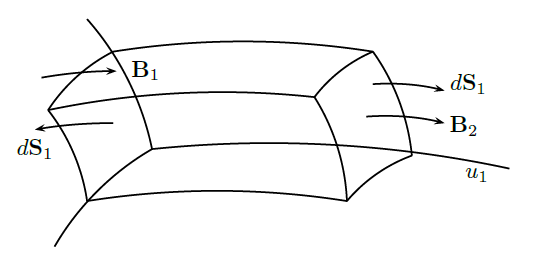
\includegraphics[scale=0.75]{Imagenes/Diferencial_Volumen.png}
    \caption{Elemento diferencial de volumen.}
    \label{fig:Diferencial_Volumen}
\end{figure}

Consideraremos el flujo total como la suma de los flujos a través de cada pareja de superficies.
\par
Como primer paso, analizamos el flujo sobre las caras $\dd{\vb{S}_{1}}$. El flujo sobre las caras $\dd{\vb{S}_{1}}$:
\begin{align*}
\dd{\Phi} &= \dd{\Phi_{u_{1} + \dd{u_{1}}}} + \dd{\Phi_{u_{1}}} \\[0.5em] 
&= \left( B_{1} \dd{S_{1}} \right)_{u_{1} + \dd{u_{1}}} - \left( B_{1} \dd{S_{1}} \right)_{u_{1}} \\[0.5em] 
&= \left( B_{1} \, h_{2} \, h_{3} \dd{u_{2}} \dd{u_{3}} \right)_{u_{1} + \dd{u_{1}}} - \left( B_{1} \, h_{2} \, h_{3} \dd{u_{2}} \dd{u_{3}} \right)_{u_{1}} \\[0.5em] 
&= \left( B_{1} \, h_{2} \, h_{3} \right)_{u_{1} + \dd{u_{1}}} \dd{u_{2}} \dd{u_{3}} - \left( B_{1} \, h_{2} \, h_{3} \right)_{u_{1}} \dd{u_{2}} \dd{u_{3}}
\end{align*}
 
Los elementos diferenciales $\dd{u_{2}} \dd{u_{3}}$ han sido extraídos del primer término, ya que son independientes de $u_{1}$.
\par
Si hacemos una expansión en serie de Taylor alrededor de $u_{1}$, tendremos:
\begin{align*}
\left( B_{1} \, h_{2} \, h_{3} \right)_{u_{1} + \dd{u_{1}}} = \left( B_{1} \, h_{2} \, h_{3} \right)_{u_{1}} + \pdv{\left( B_{1} \, h_{2} \, h_{3} \right)}{u_{1}} \dd{u_{1}} + \ldots
\end{align*}

Por lo que el flujo sobre una cara resulta:
\begin{align*}
\dd{\Phi_{1}} &= \pdv{\left( B_{1} \, h_{2} \, h_{3} \right)}{u_{1}} \dd{u_{1}} \dd{u_{2}} \dd{u_{3}} = \\[0.5em] 
&= \pdv{\left( B_{1} \, h_{2} \, h_{3} \right)}{u_{1}} \, \dfrac{\dd{V}}{h_{1} h_{2} h_{3}}
\end{align*}

De manera análoga, el flujo en las otras caras es:
\begin{align*}
\dd{\Phi_{2}} &= \pdv{\left( B_{2} \, h_{3} \, h_{1} \right)}{u_{2}} \, \dfrac{\dd{V}}{h_{1} h_{2} h_{3}} \\[1em]
\dd{\Phi_{3}} &= \pdv{\left( B_{3} \, h_{1} \, h_{2} \right)}{u_{3}} \, \dfrac{\dd{V}}{h_{1} h_{2} h_{3}}
\end{align*}

El flujo total $\dd{\Phi}$ que atraviesa el volumen $\dd{V}$ es:
\begin{align*}
\dd{\Phi} &= \dd{\Phi_{1}} + \dd{\Phi_{2}} + \dd{\Phi_{3}} = \\[1em]
&= \left[ \pdv{\left( B_{1} \, h_{2} \, h_{3} \right)}{u_{1}} + \pdv{\left( B_{2} \, h_{3} \, h_{1} \right)}{u_{2}} + \pdv{\left( B_{3} \, h_{1} \, h_{2} \right)}{u_{3}} \right] \, \dfrac{\dd{V}}{h_{1} h_{2} h_{3}}
\end{align*}

Hacemos $h \equiv h_{1} h_{2} h_{3}$, por lo que el flujo total es:
\begin{align*}
\dd{\Phi} &= \left[ \pdv{u_{1}} \left( \dfrac{B_{1} \, h}{h_{1}} \right) + \pdv{u_{2}} \left( \dfrac{B_{2} \, h}{h_{2}} \right) + \pdv{u_{3}} \left( \dfrac{B_{3} \, h}{h_{3}} \right) \right] = \\[1em]
&= {\rm Div} \, \vb{B} \dd{V}
\end{align*}

\subsubsection{Definición de divergencia.}

Se define la \emph{divergencia del campo $\vb{B}$} como la siguiente función escalar:
\begin{align}
{\rm Div} \, \vb{B} = \dfrac{1}{h} \nsum_{i=1}^{3} \pdv{u_{i}} \left( \dfrac{B_{i} \, h}{h_{i}} \right)
\label{eq:ecuacion_01_30}
\end{align}

La divergencia es el \emph{flujo por unidad de volumen}:
\begin{align*}
{\rm Div} \, \vb{B} = \dfrac{\dd{\Phi}}{\dd{V}}
\end{align*}

Este resultado se ha obtenido para una unidad de volumen diferencial.
\par
Para un volumen finito tenemos que:
\begin{align*}
\Phi = \oint \vb{B} \cdot \dd{\vb{S}}
\end{align*}
donde ya sabemos que la integración se realiza sobre una superficie \emph{cerrada}.
\par
Para calcular la integral cerrada (que equivale a sumar flujos diferenciales), se descompone el volumen $V$ en un conjunto de volúmenes diferenciales $\dd{V}$.
\par
Las caras comunes de los paralelepípedos diferenciales contribuyen con flujos iguales y opuestos en signo, que se cancelan al hacer la suma.
\par
Las partes no nulas de la integral de área son aquellas que corresponden a caras de la frontera.
\par
Por lo que:
\begin{align*}
\Phi = \oint \vb{B} \cdot \dd{\vb{S}} = \int {\rm Div} \, \vb{B} \dd{V}
\end{align*}

La integral de la divergencia sobre un volumen puede transformarse en una integral que involucra sólo el valor del campo sobre la superficie.

\subsubsection{Teorema de la divergencia.}

El resultado anterior se conoce como el \emph{Teorema de la divergencia}:
\begin{align}
\oint \vb{B} \cdot \dd{\vb{S}} = \int {\rm Div} \, \vb{B} \dd{V}
\label{eq:ecuacion_01_31}
\end{align}
La integral se extiende sobre la superficie que rodea al volumen $V$.
\par
De modo alterno tenemos que:
\begin{align*}
{\rm Div} \, \vb{B} = \lim_{\Delta V \to 0} \dfrac{\displaystyle \oint \vb{S} \dd{\vb{S}}}{\Delta V}
\end{align*}

En coordenadas curvilíneas ortogonales se tiene que:
\begin{align*}
{\rm Div} \, \vb{B} = \div{\vb{B}}
\end{align*}

El lado izquierdo de la igualdad se calcula con la ec. (\ref{eq:ecuacion_01_30}) y el lado derecho utilizando el operador gradiente de la ec. (\ref{eq:ecuacion_01_28}).
\par
% \textbf{Ejercicio a cuenta (6). } Demuestra que el campo eléctrico de una carga puntal:
% \begin{align*}
% \vb{E} = \dfrac{q \, \vu{r}}{4 \, \pi \epsilon_{0} \, r^{2}}
% \end{align*}
% cumple $\div{E} = 0$, para $r \neq 0$.
% \\[1em]
% \textbf{Ejercicio a cuenta (7). } La ley de Gauss para el campo eléctrico tiene la forma:
% \begin{align*}
% \oint \vb{E} \cdot \dd{\vb{S}} = \dfrac{q}{\epsilon_{0}}
% \end{align*}
% donde $q = \displaystyle \int \rho \dd{V}$ es la carga encerrada en la superficie y $\rho$ su densidad volumétrica.
% \par
% Demuestra la ley de Gauss en forma diferencial:
% \begin{align*}
% \div{E} = \dfrac{\rho}{\epsilon_{0}}
% \end{align*}

\subsection{Rotacional.}

\subsubsection{Circulación de un vector.}

Se define la \emph{circulación} de un vector a lo largo de una curva cerrada como:
\begin{align*}
\oint \vb{B} \cdot \dd{\vb{l}}
\end{align*}

\begin{figure}[H]
    \centering
    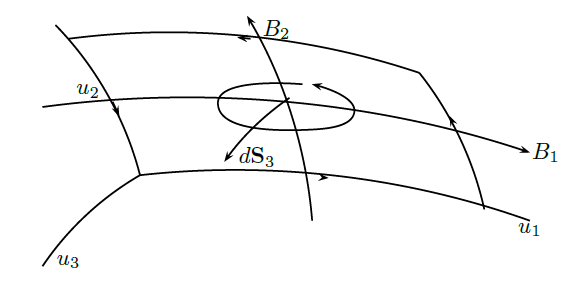
\includegraphics[scale=0.75]{Imagenes/Circulacion_Vector.png}
    \caption{Trayectoria cerrada sobre la superficie $u_{1} \, u_{3}$}
    \label{fig:figura_trayectoria_cerrada}
\end{figure}

Para el circuito diferencial de la figura (\ref{fig:figura_trayectoria_cerrada}):
\begin{align*}
\oint_{3} \vb{B} \cdot \dd{\vb{l}} &= - \left( B_{2} \dd{l_{2}} \right)_{u_{1}} + \left( B_{1} \dd{l_{1}} \right)_{u_{2}} + \\[0.5em]
&+ \left( B_{2} \dd{l_{2}} \right)_{u_{1}+\dd{u_{1}}} - \left( B_{1} \dd{l_{1}} \right)_{u_{2}+\dd{u_{2}}}
\end{align*}

Como en el caso de la divergencia, expandimos en una serie de Taylor para luego cancelar términos:
\begin{align*}
\oint_{3} \vb{B} \cdot \dd{\vb{l}} &= \left[ \displaystyle \pdv{u_{1}} \left( B_{2} \, h_{2}\right) - \pdv{u_{2}} \left( B_{1} \, h_{1} \right) \right] \dd{u_{1}} \dd_{u_{2}} = \\[0.5em] 
&= \left[ \pdv{u_{1}} \left( B_{2} \, h_{2}\right) - \pdv{u_{2}} \left( B_{1} \, h_{1} \right) \right] \, \dfrac{\dd{S_{3}}}{h_{1} h_{2}} = \\[0.5em] 
&= ({\rm{Rot}} \, \vb{B})_{3} \dd{S_{3}}
\end{align*}

El cálculo realizado ha sido considerando sólo la superficie $\dd{S_{3}}$, por lo que hay que incluir las trayectorias sobre las superficies $u_{1} = \mbox{cte.}$ y $u_{2} = \mbox{cte.}$, así tendremos:
\begin{align*}
\oint_{1} \vb{B} \cdot \dd{\vb{l}} &= ({\rm{Rot}} \, \vb{B})_{1} \dd{S_{1}} \\[1em]
\oint_{2} \vb{B} \cdot \dd{\vb{l}} &= ({\rm{Rot}} \, \vb{B})_{2} \dd{S_{2}}
\end{align*}

Los resultados anteriores consideran solo a los paralelogramos curvilíneos localizados en las superficies coordenadas.
\par
El caso general se presenta con la curva cerrada $c$ en el espacio, que rodea una superficie diferencial $\dd{\vb{S}}$.
\par
La curva cerrada se puede descomponer en $\dd{S_{1}}$, $\dd{S_{2}}$, $\dd{S_{3}}$, entonces:
\begin{align*}
\oint_{c} \vb{B} \cdot \dd{\vb{l}} = ({\rm{Rot}} \, \vb{B})_{1} \cdot \dd{S} 
\end{align*}

\subsubsection{Definición del rotacional.}

Entonces llegamos a:
\begin{align*}
{\rm Rot} \, \vb{B} &= \dfrac{\vu{e}_{1}}{h_{2} h_{3}} \left[ \displaystyle \pdv{u_{2}} \left( B_{3} \, h_{3} \right) - \pdv{u_{3}} \left( B_{2} \, h_{2} \right) \right] + \\[0.5em]
&+ \dfrac{\vu{e}_{2}}{h_{3} h_{1}} \left[ \displaystyle \pdv{u_{3}} \left( B_{1} \, h_{1} \right) - \pdv{u_{1}} \left( B_{3} \, h_{3} \right) \right] + \\[0.5em]
&+ \dfrac{\vu{e}_{3}}{h_{1} h_{2}} \left[ \displaystyle \pdv{u_{1}} \left( B_{2} \, h_{2} \right) - \pdv{u_{2}} \left( B_{1} \, h_{1} \right) \right]
\end{align*}

Ocupando el símbolo de Levi-Civita y con $h = h_{1} \, h_{2} \, h_{3}$, tenemos:
\begin{align}
\begin{aligned}
{\rm Rot} \, \vb{B} &= \dfrac{1}{h} \nsum_{i,j,k=1}^{3} \vu{e}_{i} \, \epsilon_{ijk} \, h_{i} \, \pdv{u_{j}} \left( B_{k} \, h_{k} \right) = \\[1em]
&= \nsum_{i=1}^{3} \vu{e}_{i} \left( {\rm Rot} \, \vb{B} \right)_{i}
\end{aligned}
\label{eq:ecuacion_01_34}
\end{align}

En forma matricial queda expresado como:
\begin{align*}
{\rm Rot} \vb{B} = \dfrac{1}{h_{1} \, h_{2} \, h_{3}} \mdet{
h_{1} \, \vu{e}_{1} & h_{2} \, \vu{e}_{2} & h_{3} \, \vu{e}_{3} \\[0.5em]
\displaystyle \pdv{u_{1}} & \displaystyle \pdv{u_{2}} & \displaystyle \pdv{u_{3}} \\[0.5em]
B_{1} \, h_{1} & B_{2} \, h_{2} & B_{3} \, h_{3}
}
\end{align*}
El operador $\pdv*{u_{i}}$ opera solo sobre la tercera fila. Es posible demostrar que:
\begin{align*}
{\rm Rot} \, \vb{B} = \curl{B}
\end{align*}

De la expresión:
\begin{align*}
\oint_{c} \vb{B} \cdot \dd{\vb{l}} = (\curl{B}) \cdot \dd{\vb{S}}
\end{align*}
se sigue que:
\begin{align*}
\oint \vb{B} \cdot \dd{\vb{l}} = \abs{\curl{B}} \dd{S \, \cos \theta}
\end{align*}

La máxima circulación se obtiene con $\theta = 0$,
\begin{align*}
\left( \dfrac{\displaystyle \oint \vb{B} \cdot \dd{\vb{l}}}{\dd{S}} \right)_{\max} = \abs{\curl{\vb{B}}}
\end{align*}
Es decir: \emph{el módulo del rotacional es la máxima circulación por unidad de área}.

\subsubsection{Teorema de Stokes.}

Los cálculos que se han realizado son válidos para un circuito diferencial.
\par
En el caso de una curva cerrada que encierre una superficie abierta finita, se tendrán que sumar sobre el conjunto de circuitos elementales, como se muestra en la siguiente figura (\ref{fig:figura_superficie_elementos_diferenciables})

\begin{figure}[H]
    \centering
    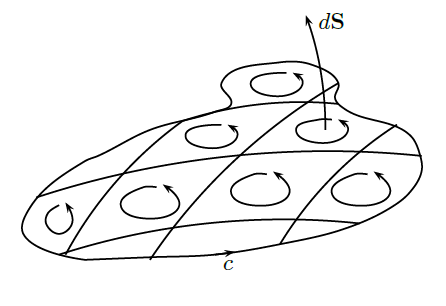
\includegraphics[scale=0.75]{Imagenes/Superficie_Elementos_Diferenciables.png}
    \caption{Descomposición de una superficie finita en elementos diferenciables.}
    \label{fig:figura_superficie_elementos_diferenciables}
\end{figure}

Los circuitos con lados comunes no contribuyen a la circulación.
\par
La contribución neta se debe solo a los elementos de línea ubicados en el contorno $c$. Entonces tenemos:
\begin{align}
\oint_{c} \vb{B} \cdot \dd{\vb{l}} = \int_{S} \curl{\vb{B}} \cdot \dd{\vb{S}}
\label{eq:ecuacion_01_35}
\end{align}
Que conocemos con el \emph{Teorema de Stokes}, que nos permite reemplazar integrales de área por integrales de línea.
% \\[1em]
% \textbf{Ejercicio a cuenta (8). } Demuestra que:
% \begin{align*}
% \curl(\phi \, \vb{A}) = \phi \, \curl{\vb{A}} + \grad{\phi} \times \vb{A}
% \end{align*}
% \\[1em]
% \textbf{Ejercicio a cuenta (9). } El campo electrostático de un dipolo eléctrico $\vb{p} = p_{0} \, \vu{e}_{z}$ es:
% \begin{align*}
% \vb{E} = \dfrac{p_{0} (2 \, \vu{e}_{r} \, \cos \theta + \vu{e}_{\theta} \, \sin \theta)}{r^{3}}
% \end{align*}
% Demuestra que:
% \begin{enumerate}
% \item $\curl{\vb{E}} = 0$
% \item para $r \neq 0$, se tiene $\div{\vb{E}} = 0$
% \end{enumerate}

\subsection{Laplaciano.}

\subsubsection{Definición.}

El Laplaciano de una función escalar $f(u_{i})$, que se representa por $\laplacian{f(u_{i})}$, se define como:
\begin{align*}
\laplacian{f} = \div{\nabla f}
\end{align*}

Entonces por la ec. (\ref{eq:ecuacion_01_30}), con $B_{i} = (\nabla f)$:
\begin{align*}
\laplacian{f} = \dfrac{1}{h} \, \nsum_{i=1}^{3} \pdv{u_{i}} \left( \dfrac{h}{h_{i}}  (\nabla f)_{i} \right)
\end{align*}

De acuerdo con la ec. (\ref{eq:ecuacion_01_28}):
\begin{align*}
(\nabla f) = \dfrac{1}{h_{i}} \pdv{f}{u_{i}}
\end{align*}

Se sigue entonces que:
\begin{align}
\laplacian{f} = \dfrac{1}{h} \, \nsum_{i=1}^{3} \pdv{u_{i}} \left( \dfrac{h}{h_{i}^{2}}  \pdv{f}{u_{i}} \right)
\label{eq:ecuacion_01_36}
\end{align}

\subsubsection{Laplaciano en coordenadas ortogonales.}

El Laplaciano en coordenadas cartesianas, cilíndricas y esféricas, respectivamente es:
\begin{align}
\laplacian{f} &= \pdv[2]{f}{x} + \pdv[2]{f}{y} + \pdv[2]{f}{z} \label{eq:laplaciano_cartesianas} \\[1em]
\laplacian{f} &= \dfrac{1}{\rho} \, \pdv{\rho} \left( \rho \, \pdv{f}{\rho} \right) + \dfrac{1}{\rho^{2}} \, \pdv[2]{f}{\varphi} + \pdv[2]{f}{z} \label{eq:laplaciano_cilindricas}\\[1em]
\laplacian{f} &= \dfrac{1}{r^{2}} \pdv{r} \left( r^{2} \pdv{f}{r} \right) + \dfrac{1}{r^{2} \sin \theta} \, \pdv{\theta} \left( \sin \theta \pdv{f}{\theta} \right) + \dfrac{1}{r^{2} \, \sin^{2} \theta} \, \pdv[2]{f}{\varphi} \label{eq:laplaciano_esfericas}
\end{align}
% \\[1em]
% \textbf{Ejercicio a cuenta (10). } Demuestra que el Laplaciano en coordenadas cilíndricas y esféricas es el que se presenta en las ecs. (\ref{eq:laplaciano_cilindricas}) y (\ref{eq:laplaciano_esfericas}) respectivamente, para ello tendrás que calcular los correspondientes factores de escala.

\subsection{Laplaciano de una función vectorial.}

En otros sistemas de coordenadas, el Laplaciano de una función vectorial se define por:
\begin{align*}
\laplacian{\vb{A}} = \grad{(\div{A})} - \curl{(\curl{\vb{A}})}
\end{align*}

\subsection{El Laplaciano en la física.}

El Laplaciano se encontrará en distintas áreas de la física: electrostática, magnetostática, gravitación, flujo de fluidos, mecánica cuántica, difusión de calor entre otros.
\par
El tipo más sencillo de campo vectorial $\vb{F}(\vb{r})$ es donde el campo es irrotacional, incompresible (llamado también de divergencia nula), continuo y derivable.
\par
Por ser un campo irrotacional, donde $\curl{\vb{F}} = 0$, existe un potencial $\phi$, tal que:
\begin{align*}
\vb{F} = \grad{\phi}
\end{align*}

Por ser un campo incompresible, donde $\div{\vb{F}} = 0$, entonces:
\begin{align*}
\laplacian{\phi} = 0
\end{align*}

La solución a la ecuación de Laplace se denomina \emph{función armónica}.
\par
El potencial de un campo electrostático es armónico en el exterior de las cargas; mientras que en un fluido de densidad constante, el potencial de velocidad es armónico, si no hay fuentes ni sumideros.

\section{Utilidad de los operadores.}

\subsection{Expresión de ecuaciones diferenciales.}

Con la construcción que hemos revisado, ahora tenemos la oportunidad de expresar fenómenos físicos en algún sistema coordenado particular, de tal manera que si están involucrados los operadores diferenciales, la ecuación resultante será más fácil de manejar.

Una vez que hayamos expresado la ecuación diferencial, el siguiente paso será resolverla. Para ello, revisaremos algunas técnicas de solución que se trabajarán en el \emph{\textcolor{blue}{Tema 2 - Primeras técnicas de solución}}.

\subsection{La ecuación de Helmholtz.}

La ecuación de Helmholtz:
\begin{align}
\nabla^{2} \psi + k^{2} \: \psi = 0
\label{eq:ecuacion_02_01}
\end{align}
es una ecuación separable. Diremos que una ecuación es separable cuando la solución de la misma $\psi(x, y, z)$, se expresa como el producto de funciones que dependen solo de una variable: $\psi(x, y, z) = X (x) \, Y (y),\, Z(z)$, logrando con ello un paso importante en el cambio de tipo de ecuación diferencial parcial a un sistema de ecuaciones diferenciales ordinarias, que ya podremos resolver de manera más sencilla y directa. 
\par
Como primer paso para \emph{separar} una ecuación, se debe de reescribir la misma en el sistema coordenado de interés, ocupando los correspondientes operadores diferenciales que intervengan.
\par
En particular, la ecuación de Helmholtz tiene el hecho de que si:
\begin{itemize}
\item $k^{2} = 0$, se obtiene la ecuación de Laplace.
\item $k^{2} = (+) \mbox{ constante}$, se obtiene la ecuación de Helmholtz.
\item $k^{2} = (-) \mbox{ constante}$, se obtiene la ecuación de difusión (en su parte espacial).
\item $k^{2} = \mbox{ constante } \times \mbox{ energía cinética}$, se obtiene la ecuación de onda de Schrödinger.
\end{itemize}

Se ha demostrado que existen once sistemas coordenados en donde la ecuación de Helmholtz  (ec. \ref{eq:ecuacion_02_01}) puede separarse. 
\par
\textbf{Importante: } Cabe señalar que en algunos textos se ocupa una notación para las nuevas coordenadas con letras del alfabeto castellano: $(u, v, w)$.
\par
Otros textos ocupan letras griegas: $(\xi, \eta, \mu, \nu, \theta, \psi, \phi, \lambda, \varphi)$.
\par
Sin pérdida de generalidad, ocupar cualquiera de las notaciones indicadas representa lo mismo. Lo importante es trabajar con las reglas de transformación. A continuación se presenta la ecuación de Helmholtz en algunos sistemas coordenados\footnote{Si en algún ejercicio se pide la expresión de esta ecuación, pero que no se haya desarrollado de manera explícita, deberán de hacer el trabajo de obtener los respectivos factores de escala, obtener el operador diferencial laplaciano y escribir la ecuación, ya sea la de Helmholtz o cualquier otra de la Física Matemática. Las expresiones que se muestran en la lista se entiende que \emph{no están desarrolladas de manera explícita.}}, convendría que realices las operaciones necesarias para lograr la expresión que se indica.
\par
\begin{enumerate}
\item Coordenadas cilíndricas circulares $(\rho, \phi, z)$.
\begin{align*}
\dfrac{1}{\rho} \pdv{\rho} \bigg( \rho \pdv{\psi}{\rho} \bigg) + \dfrac{1}{\rho^{2}} \pdv[2]{\phi}{\varphi} + \pdv[2]{\psi}{z} + k^{2} \, \psi = 0
\end{align*}
\item Coordenadas cilíndricas elípticas $(u, v, z)$.
\begin{align*}
\dfrac{1}{a \big( \sinh^{2} u + \sin^{2} v \big)} \bigg( \pdv[2]{\psi}{u} + \pdv[2]{\psi}{v} \bigg) + \pdv[2]{\psi}{z} + k^{2} \, \psi = 0
\end{align*}
\item Coordenadas cilíndricas elípticas $(u, v, z)$.
\begin{align*}
\dfrac{1}{u^{2} + v^{2}} \bigg( \pdv[2]{\psi}{u} + \pdv[2]{\psi}{v} \bigg) + \pdv[2]{\psi}{z} + k^{2} \, \psi = 0
\end{align*}
\item Coordenadas esféricas polares $(\rho, \theta, \phi)$.
\begin{align*}
\dfrac{1}{r^{2}} \pdv{r} \bigg( r^{2} \pdv{\psi}{r} \bigg) + \dfrac{1}{r^{2} \sin \theta} \pdv{\theta} \bigg( \sin \pdv{\psi}{\theta} \bigg) + \dfrac{1}{r^{2} \sin^{2} \theta} \pdv[2]{\psi}{\varphi} + k^{2} \, E = 0
\end{align*}
\item Coordenadas esferoidales prolatas $(\xi, \eta, \phi)$.
\begin{align*}
&\dfrac{1}{\sinh \xi} \pdv{\xi} \bigg( \sinh \xi \pdv{\psi}{\xi} \bigg) + \dfrac{1}{\sin \eta} \pdv{\eta} \bigg( \sin \eta \pdv{\psi}{\eta} \bigg) + \\[0.5em]
&+ \bigg( \dfrac{\sinh^{2} \xi + \sin^{2} \eta}{\sinh^{2} \xi \, \sin^{2} \eta} \bigg) \pdv[2]{\psi}{\phi} + k^{2} a^{2} (\sinh^{2} \xi + \sin^{2} \eta) = 0
\end{align*}
\item Coordenadas esferoidales oblatas $(\xi, \eta, \phi)$.
\begin{align*}
&\dfrac{1}{\cosh \xi} \pdv{\xi} \bigg( \cosh \xi \pdv{\psi}{\xi} \bigg) + \dfrac{1}{\sin \eta} \pdv{\eta} \bigg( \sin \eta \pdv{\psi}{\eta} \bigg) + \\[0.5em]
&+ \bigg( \dfrac{\cosh^{2} \xi - \sin^{2} \eta}{\cosh^{2} \xi \, \sin^{2} \eta} \bigg) \pdv[2]{\psi}{\phi} + k^{2} a^{2} (\cosh^{2} \xi - \sin^{2} \eta) = 0
\end{align*}
\item Coordenadas parabólicas $(u, v, \phi)$.
\begin{align*}
\dfrac{1}{u (u^{2} + v^{2})} \pdv{u} \bigg( u \pdv{\psi}{u} \bigg) + \dfrac{1}{v (u^{2} + v^{2})} \pdv{v} \bigg( v  \pdv{\psi}{v} \bigg) + \dfrac{1}{u^{2} v^{2}} \pdv[2]{\psi}{\phi} +k^{2} \, E = 0
\end{align*}
\end{enumerate}
\end{document}